\documentclass{article}

\usepackage[utf8]{inputenc}
\usepackage[frenchb]{babel}

\usepackage{hyperref}
\usepackage{graphicx}

\usepackage{listings}
\lstdefinestyle{customstyle}{
    basicstyle=\footnotesize,
    breakatwhitespace=false,         
    breaklines=true,                 
    captionpos=b,                    
    keepspaces=true,                                                                                       
    tabsize=4,
    frame=single, %lines
    moredelim=[is][\underbar]{_}{_} % underlines permitted without escape character
}
\lstset{style=customstyle}

\title{Free Basic to C compiler}
\author{Jérémy Bardon}

\begin{document}
	\maketitle

	\section{Introduction}
Le but de ce projet est de créer un compilateur capable de convertir un code écrit 
en \href{http://www.freebasic.net}{Free Basic} dans le langage C. 

\begin{figure}[h]
    \centering
    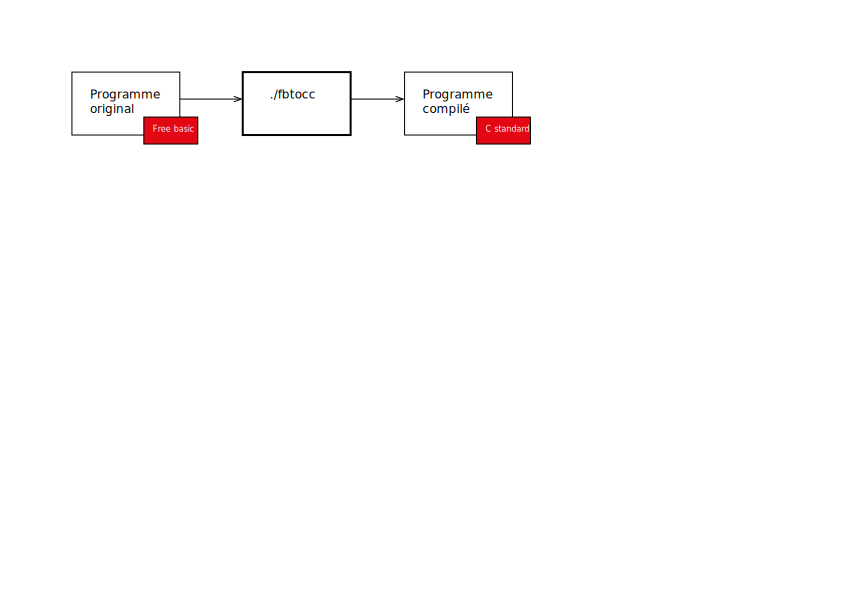
\includegraphics[scale=0.6]{schema.png}
    \caption{Rôle du compilateur}
\end{figure}
	
Le programme en C
ainsi généré sera compilable avec \emph{gcc} et effectuera les mêmes opérations que 
le programme original.
	
	\section{Adaptations}
Par défaut, un programme écrit en free basic dispose comme en C d'un 
certain nombre de fonctions que l'on peut utiliser sans inclure des programmes 
externes. Cependant, ces fonctions \og{}basiques\fg{} ne sont pas équivalentes dans 
les deux langages.
\\\\
L'exemple le plus simple est la fonction qui permet d'afficher un message : en 
free basic il s'agit de la fonction \emph{print} qui est incluse 
par défaut mais en C il est nécessaire d'inclure \emph{stdio.h}.
\\\\
Une autre différence de taille est la présence -- en C -- d'une routine principale 
(main) qui doit être présente dans tout programme écrit en C. Ce n'est pas le cas du 
free basic qui propose une structure plus libre du programme.
\newpage
\lstset{language=c,caption=Programme C englobant}
\lstinputlisting{wrap.c}

Ce sont ces différences qui amènent à devoir proposer une structure englobante d'un 
programme dans laquelle on va ensuite insérer le code free basic converti.
	
	\section{Fonctionnalités implémentées}
\begin{itemize}
\item Fonction à 1 argument (affichage d'un message)
\item Déclaration de constantes (entier et chaîne de caractères)
\item Déclaration et changement de valeur de variables (entier et chaîne de caractères)
\item Commentaire mono-ligne
\item Condition simple (pas de close sinon)
\item Report du numéro de ligne et de caractère en cas d'erreur lors du parsing
\end{itemize}	
	
	\section{Grammaire}
	\section{Reconnaissance des erreurs}
	
\end{document}